% Copyright (c) 2017 Aleksa Sarai <asarai@suse.de>
% This work is licensed under the Creative Commons Attribution-ShareAlike 4.0
% International License. To view a copy of this license, visit
% http://creativecommons.org/licenses/by-sa/4.0/ or send a letter to Creative
% Commons, PO Box 1866, Mountain View, CA 94042, USA.

\documentclass[10pt,aspectratio=169]{beamer}
\usetheme{metropolis}
\metroset{background=light}
\metroset{titleformat=smallcaps}

\usepackage{pbox}
\usepackage{fontspec}
\usepackage[absolute,overlay]{textpos}
\usepackage[math-style=TeX]{unicode-math}
\usepackage{booktabs}

\usepackage{tikz}
\usetikzlibrary{calc}

\usepackage{hyperref}
\usepackage{graphicx}
\graphicspath{{.}{assets/}}

\setbeamertemplate{caption}{\raggedright\insertcaption\par}

\title{Rootless Containers with runC}
\author{%
		Aleksa Sarai \\
		Software Engineer \\
		SUSE Linux GmbH \\
		\href{mailto:asarai@suse.de}{\tiny\tt \underline{asarai@suse.de}}}

\date{}
\institute{}

\begin{document}
	\begin{frame}[plain,noframenumbering]
		\begin{tikzpicture}[remember picture,overlay]
			\node[anchor=north east] at ($(current page.north east) - (-0.3, 0.3)$) {
\includegraphics[height=2cm]{man-in-business-suit-levitating}};
			\node[anchor=south east] at ($(current page.south east) + (-0.3, 0.3)$) {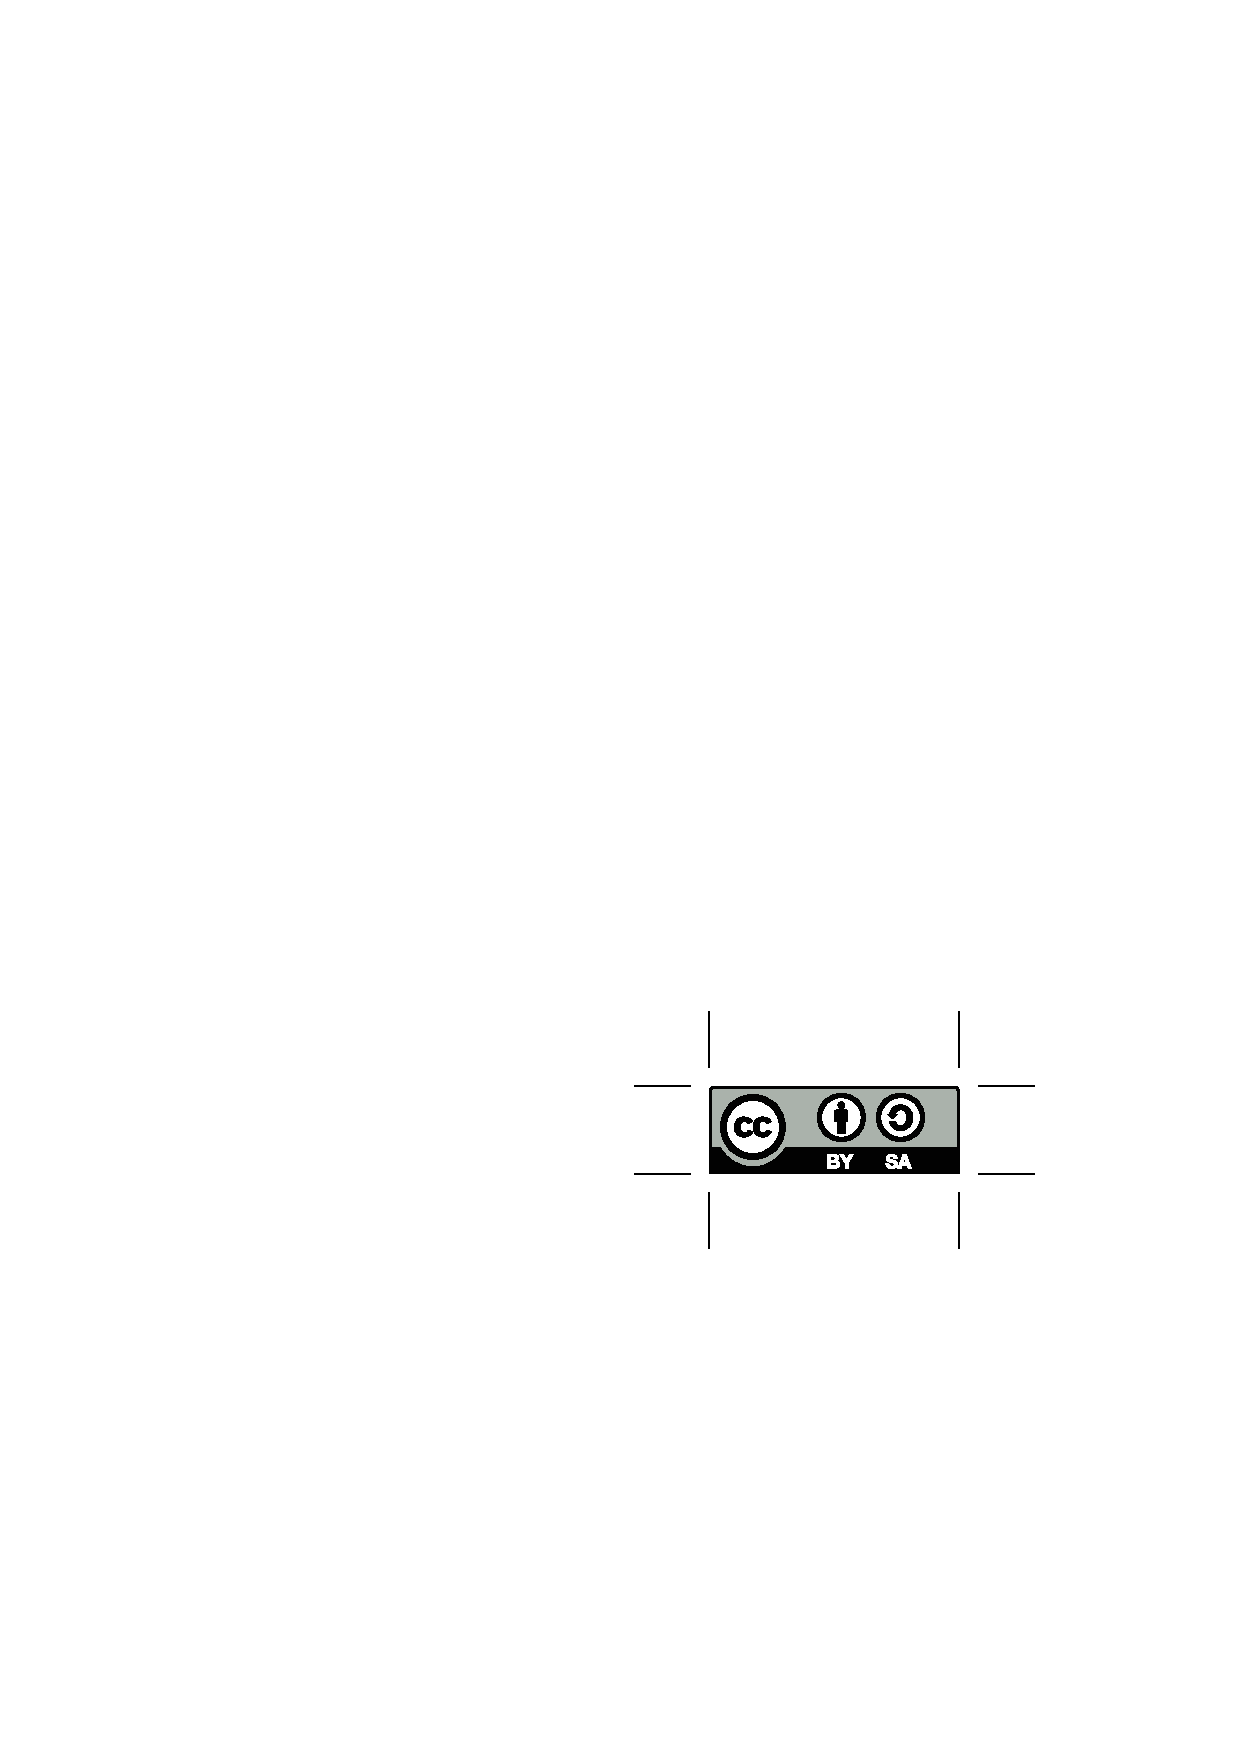
\includegraphics[width=1.2cm]{cc_by_sa}};
			\node[anchor=south west] at ($(current page.south west) + (2.3, 0.3)$) {
\includegraphics[height=0.6cm]{oci_logo}};
			\node[anchor=south west] at ($(current page.south west) + (0.3, 0.3)$) {
\includegraphics[height=0.75cm]{suse_logo}};
		\end{tikzpicture}

		\titlepage%
	\end{frame}

	\begin{frame}{\texttt{whoami}}
		\begin{itemize}
			\item Aleksa Sarai $\to$ \texttt{\small cyphar}
			\item Software Engineer on the Containers team at SUSE\@.
			\item Undergraduate student at the University of Sydney.
			\item runC maintainer.
			\item Long-term contributor to the Open Container Initiative and Docker.
			\item Proponent of Free Software.
		\end{itemize}
	\end{frame}

	\begin{frame}{Open Container Initiative}
		\begin{itemize}
			\item Standards body created in $2015$ to standardise container formats and runtimes.
			\item Two main components:
			\begin{itemize}
				\item Runtime configuration.
				\item Image format.
			\end{itemize}
			\item runC is the de-facto implementation of the runtime specification.
			\begin{itemize}
				\item It just needs a root filesystem and configuration file.
			\end{itemize}
			\item \dots~and it's the runtime used by Docker.
		\end{itemize}
	\end{frame}

	\begin{frame}{A Hypothetical Researcher \dots}
		\begin{itemize}
			\item Researcher wants to run Python 3 code on a Python 2 cluster.
			\item<2-> So they use a container to package Python 3 --- right?
			\begin{itemize}
				\item<2-> But the administrator (quite rightly) doesn't want to install ``new-fangled software''.
			\end{itemize}
			\item<3-> Okay, so they compile all of the dependencies from scratch --- right?
			\begin{itemize}
				\item<3-> \textit{Ha, ha.}
			\end{itemize}
			\item<4-> What should our researcher do?
			\begin{itemize}
				\item<4-> What if we could create and run containers without privileges?
			\end{itemize}
			\item<5-> Not actually a hypothetical --- this was me in early $2016$.
			\item<5-> \dots~and many other researchers have this problem.
		\end{itemize}
	\end{frame}

	\begin{frame}{How do we do that?}
		\begin{itemize}
			\item Containers are mostly made of Linux kernel namespaces.
			\begin{itemize}
				\item \texttt{cgroup}s are not actually required.
				\item Oh, and it's mostly duct tape and hacks.
			\end{itemize}
			\item They isolate a process's view of parts of the system.
			\item One of the most interesting namespaces is the \texttt{USER} namespace.
			\begin{itemize}
				\item You can ``pretend'' that an unprivileged user is root.
			\end{itemize}
		\end{itemize}
	\end{frame}

	\begin{frame}{\texttt{USER} Namespaces}
		\begin{itemize}
			\item Capabilities and uids are scoped to their \texttt{USER} namespace.
			\item Permission checks are done based on the namespaces a process is in.
			\item Based on mapping the host's \texttt{uid}s and \texttt{gid}s into the container.
			\item \texttt{EPERM} on all operations on \textbf{unmapped} \texttt{uid}s or \texttt{gid}s.
		\end{itemize}
	\end{frame}

	\begin{frame}{Unprivileged \texttt{USER} Namespaces}
		\begin{itemize}
			\item Since Linux $3.8$, unprivileged users can create new \texttt{USER} namespaces.
			\begin{itemize}
				\item And it's been \textit{mostly} safe since Linux $3.19$.
			\end{itemize}
			\item All other namespaces are ``owned'' by a given \texttt{USER} namespace.
			\begin{itemize}
				\item You can create a fully namespaced environment without privileges!
				\item Operations in these namespaces are more restricted than usual.
			\end{itemize}
			\item Only your user and group are mapped!
		\end{itemize}
	\end{frame}

	\begin{frame}{Implementing it!}
		\begin{itemize}
			\item Get a container runtime to implement this for you!
			\begin{itemize}
				\item<2-> \dots~which I've already done for you!
			\end{itemize}
			\item<2-> \dots~or you could do it manually:
			\begin{itemize}
				\tt
				\item<3-> {unshare -UrmunipCf bash}
				\item<3-> {mount --make-rprivate / \&\& mount --rbind rootfs/ rootfs/}
				\item<3-> {mount -t proc proc rootfs/proc}
				\item<3-> {mount -t tmpfs tmpfs rootfs/dev}
				\item<3-> {mount -t devpts -o newinstance devpts rootfs/dev/pts}
				\item<3-> {\#~\dots~skipping over a lot more mounting~\dots}
				\item<3-> {pivot\_root rootfs/ rootfs/.pivot\_root \&\& cd /}
				\item<3-> {mount --make-rprivate /.pivot\_root \&\& umount -l /.pivot\_root}
				\item<3-> {exec bash \# finally}
			\end{itemize}
		\end{itemize}
	\end{frame}

	\begin{frame}{What works?}
		\begin{itemize}
			\item All basic functionality works with rootless containers.
			\begin{itemize}
				\item \underline{\url{https://github.com/opencontainers/runc/pull/774}}
				\item \dots~and it's all tested!
			\end{itemize}
		\end{itemize}

		\vfill

		\begin{center}
			\tt
			\begin{tabular}{rl}
				\textnormal{Works} & \textnormal{Broken} \\
				\toprule
				run & checkpoint \textit{\textnormal{[criu]}}\\
				exec & restore \textit{\textnormal{[criu]}} \\
				kill & pause \textit{\textnormal{[cgroups]}} \\
				delete & resume \textit{\textnormal{[cgroups]}} \\
				list & events \textit{\textnormal{[cgroups]}} \\
				state & ps \textit{\textnormal{[cgroups]}} \\
				spec & \\
				create & \\
				start & \\
				--detach & \\
			\end{tabular}
		\end{center}
	\end{frame}

	\begin{frame}{What about images?}
		\begin{itemize}
			\item Runtime is only half of the story --- what about images?
			\item Recently, two tools have been created to make this very easy.
			\begin{description}
				\item[\href{https://github.com/projectatomic/skopeo}{\underline{skopeo}}] Download and convert images from various sources and registries.
				\item[\href{https://github.com/cyphar/umoci}{\underline{umoci}}] Unpack, repack and otherwise modify local OCI images.
			\end{description}
			\item Now you can use images as an unprivileged user too!
			\begin{itemize}
				\item You don't get cool filesystem features though.
			\end{itemize}
		\end{itemize}
	\end{frame}

	\begin{frame}
		\begin{tikzpicture}[remember picture,overlay]
			\node[anchor=north east] at (current page.north east) {
\includegraphics[width=3.5cm]{runc_hamster}};
		\end{tikzpicture}

		\begin{center}
			\Huge Live Demo!
		\end{center}
		\begin{center}
			May the demo gods have mercy.
		\end{center}
	\end{frame}

	\begin{frame}{\texttt{remainroot}\@(1)}
		\begin{itemize}
			\item Certain syscalls will \textbf{always} fail inside a rootless container.
			\begin{itemize}
				\item \texttt{setuid}\@(2), \texttt{setgid}\@(2), \texttt{chown}\@(2), \texttt{setgroups}\@(2), \texttt{mknod}\@(2), etc.
			\end{itemize}
			\item Others will give confusing results.
			\begin{itemize}
				\item \texttt{getgroups}\@(2), \texttt{waitid}\@(2), etc.
			\end{itemize}
			\item Package managers will therefore fail to ``drop privileges''.
			\item \textit{Solution}: Write a tool to emulate GNU/Linux's privilege model using \texttt{ptrace}\@(2).
			\begin{itemize}
				\item It currently \textit{sort of} works, but requires more shims and testing.
				\item \underline{\url{https://github.com/cyphar/remainroot}}
			\end{itemize}
		\end{itemize}
	\end{frame}

	\begin{frame}{What about networking?}
		\begin{itemize}
			\item Unprivileged \texttt{NET} namespaces aren't useful.
			\begin{itemize}
				\item They only have a loopback interface.
			\end{itemize}
			\item To create \texttt{veth} pairs you need \texttt{CAP\_NET\_ADMIN} in both \texttt{NET} namespaces.
			\item \textit{Solution}: Don't set up the \texttt{NET} namespace and just use the \textbf{host} namespace like a normal process.
			\begin{itemize}
				\item Which means you don't get to use \texttt{iptables}\@(8).
				\item \dots~but at least you get network access!
			\end{itemize}
			\item But there is some movement in the kernel to fix this problem.
		\end{itemize}
	\end{frame}

	\begin{frame}{What about \texttt{cgroup}s?}
		\begin{itemize}
			\item \texttt{cgroup}s are a resource control mechanism.
			\item \texttt{cgroup}s interface is effectively a virtual filesystem.
			\begin{itemize}
				\item Everything under \texttt{/sys/fs/cgroup} is owned by \texttt{root} and \texttt{chmod go-w}.
			\end{itemize}
			\item But most \texttt{cgroupv1} controllers are hierarchical!
			\begin{itemize}
				\item And \texttt{cgroupv2} is entirely hierarchical, by design.
				\item So why don't we have unprivileged subtree management?
			\end{itemize}
			\item \textit{Solution}: Submit kernel patches that implement unprivileged subtree management.
			\begin{itemize}
				\item Currently at version $10$ of the patch set.
				\item Maintainer doesn't seem to like the idea at all.
			\end{itemize}
		\end{itemize}
	\end{frame}

	\begin{frame}{What other stuff is broken?}
		\begin{itemize}
			\item I just found out that the fix for \texttt{CVE-\@2016-\@9962} broke rootless containers.
			\begin{itemize}
				\item It was a kernel bug, sent a patch yesterday.
				\item \dots~the point being the interfaces are still janky.
			\end{itemize}
			\item \texttt{runc ps} uses \texttt{cgroup}s but we could potentially implement it differently.
			\begin{itemize}
				\item Unfortunately tricky because it requires \texttt{AF\_UNIX} socket magic.
			\end{itemize}
			\item \textit{Please} test this code and tell me what you find!
			\begin{itemize}
				\item \underline{\url{https://github.com/opencontainers/runc/pull/774}}
			\end{itemize}
		\end{itemize}
	\end{frame}

	\begin{frame}{Just for Researchers?}
		\begin{itemize}
			\item Researchers are not the only target!
			\item What if you could use container features in desktop applications?
			\begin{itemize}
				\item \dots~or start Kubernetes as part of an application?
				\item \dots~or build images in a build system without privileges?
				\item \dots~or \textit{<insert your idea here>}
				\item \dots~or \textbf{PROFIT!}
			\end{itemize}
		\end{itemize}
	\end{frame}

	\begin{frame}{Future of Free Software?}
		\begin{itemize}
			\item Back to the theme of the conference: ``The Future of Free Software''.
			\item In my mind the future is refining and extending existing ideas.
			\begin{itemize}
				\item In containers, this is allowing everyone to use them.
			\end{itemize}
			\item But more importantly, the future is \textbf{what we make it}.
		\end{itemize}
	\end{frame}

	\begin{frame}{Acknowledgements}
		\begin{itemize}
			\item \textbf{Jessie Frazelle} --- started working on this first and inspired me with her PoC, \href{https://github.com/jessfraz/binctr}{\underline{binctr}}.
			\item \textbf{Eric Biederman}  --- working tirelessly to get \texttt{USER} namespaces working.
			\item \textbf{James Bottomley} --- helped me with kernel patches trying to fix the \texttt{cgroup} issue.
		\end{itemize}
	\end{frame}

	\begin{frame}
		\begin{center}
			\Huge Questions?
		\end{center}
	\end{frame}
\end{document}
